\documentclass[../notes.tex]{subfiles}

\pagestyle{main}
\renewcommand{\chaptermark}[1]{\markboth{\chaptername\ \thechapter\ (#1)}{}}
\stepcounter{chapter}

\begin{document}




\chapter{Solving Simple ODEs}
\section{Separable ODEs}
\begin{itemize}
    \item \marginnote{10/3:}Do not sit on the left side of the classroom: The sun sucks!
    \item \textbf{Separable} (ODE): An ODE of the form
    \begin{equation*}
        \dv{y}{t} = f(t)g(y)
    \end{equation*}
    where $y$ is a real\footnote{We may come back to complex functions later.}, unknown, scalar function of $t$.
    \item Solving separable ODEs: Formally, evaluate
    \begin{equation*}
        \int\frac{\dd{y}}{g(y)} = \int f(t)\dd{t}
    \end{equation*}
    \begin{itemize}
        \item But how do we know that we can move the Liebniz notation around so conveniently?
    \end{itemize}
    \item Proving the validity of the above formula.
    \begin{itemize}
        \item Rearrange the initial separable ODE to $\dv*{y}{t}\cdot 1/g=f$ and invoke the law of composite differentiation to get
        \begin{equation*}
            \dv{t}\left[ \int_{y_0}^{y(t)}\frac{\dd{w}}{g(w)}-\int_{t_0}^tf(\tau)\dd{\tau} \right] = 0
        \end{equation*}
        \item It follows that
        \begin{equation*}
            \int_{y_0}^{y(t)}\frac{\dd{w}}{g(w)} = \int_{t_0}^tf(\tau)\dd{\tau}
        \end{equation*}
        \item Ask about this in OH??
    \end{itemize}
    \item Examples:
    \begin{enumerate}
        \item Exponential growth.
        \begin{itemize}
            \item We have that
            \begin{equation*}
                \dv{y}{t} = ky
            \end{equation*}
            for $k>0$ and $y(0)=y_0>0$.
            \item The solution is
            \begin{align*}
                \frac{1}{y}\cdot\dv{y}{t} &= k\\
                \log y(t)-\log y_0 &= kt\\
                y(t) &= y_0\e[kt]
            \end{align*}
        \end{itemize}
        \item Logistic growth.
        \begin{itemize}
            \item We have that
            \begin{equation*}
                \dv{y}{t} = ky\left( 1-\frac{y}{M} \right)
            \end{equation*}
            for $k,M>0$ and $y(0)=y_0>0$.
            \item The solution is
            \begin{align*}
                \frac{M\dd{y}}{y(M-y)} &= k\dd{t}\\
                \log\frac{y}{M-y}-\log\frac{y_0}{M-y_0} &= kt\\
                \frac{y(M-y_0)}{y_0(M-y)} &= \e[kt]\\
                y\cdot\frac{M-y_0}{y_0} &= (M-y)\e[kt]\\
                y\cdot\frac{M-y_0}{y_0}+y\e[kt] &= M\e[kt]\\
                y\left( \frac{M-y_0}{y_0}+\e[kt] \right) &= M\e[kt]\\
                y\left( \frac{M-y_0+y_0\e[kt]}{y_0} \right) &= M\e[kt]\\
                y\left( \frac{M+y_0(\e[kt]-1)}{y_0} \right) &= M\e[kt]\\
                y(t) &= \frac{My_0\e[kt]}{M+y_0(\e[kt]-1)}
            \end{align*}
            \item Sketches the graph of logistic growth and discusses the turning point (for which there is a formula; zero of the second derivative) as well as general trends.
            \item If $y_0<0$, the solution is not physically meaningful, but it is mathematically insightful.
            \begin{itemize}
                \item When we integrate, the arguments of our logarithms now have absolute values.
                \begin{equation*}
                    \log\left| \frac{y}{M-y} \right|-\log\left| \frac{y_0}{M-y_0} \right| = kt
                \end{equation*}
                \item We need to make sure that the denominator of the final logistic form is never equal to zero, but now that $y_0$ is negative, as $t$ increases, the denominator will approach zero exponentially. It reaches zero when
                \begin{align*}
                    M+y_0(\e[kt]-1) &= 0\\
                    \e[kt] &= -\frac{M}{y_0}+1
                \end{align*}
                In other words, $t_\text{max}=(1/k)\log(1-M/y_0)$; when $t=t_\text{max}$, the equation blows up.
                \item This is an example of \textbf{finite lifespan}.
            \end{itemize}
            \item If $y_0>M$, then you will exponentially (really??) decrease to $M$.
        \end{itemize}
        \item Lotka-Volterra predator-prey model.
        \begin{figure}[H]
            \centering
            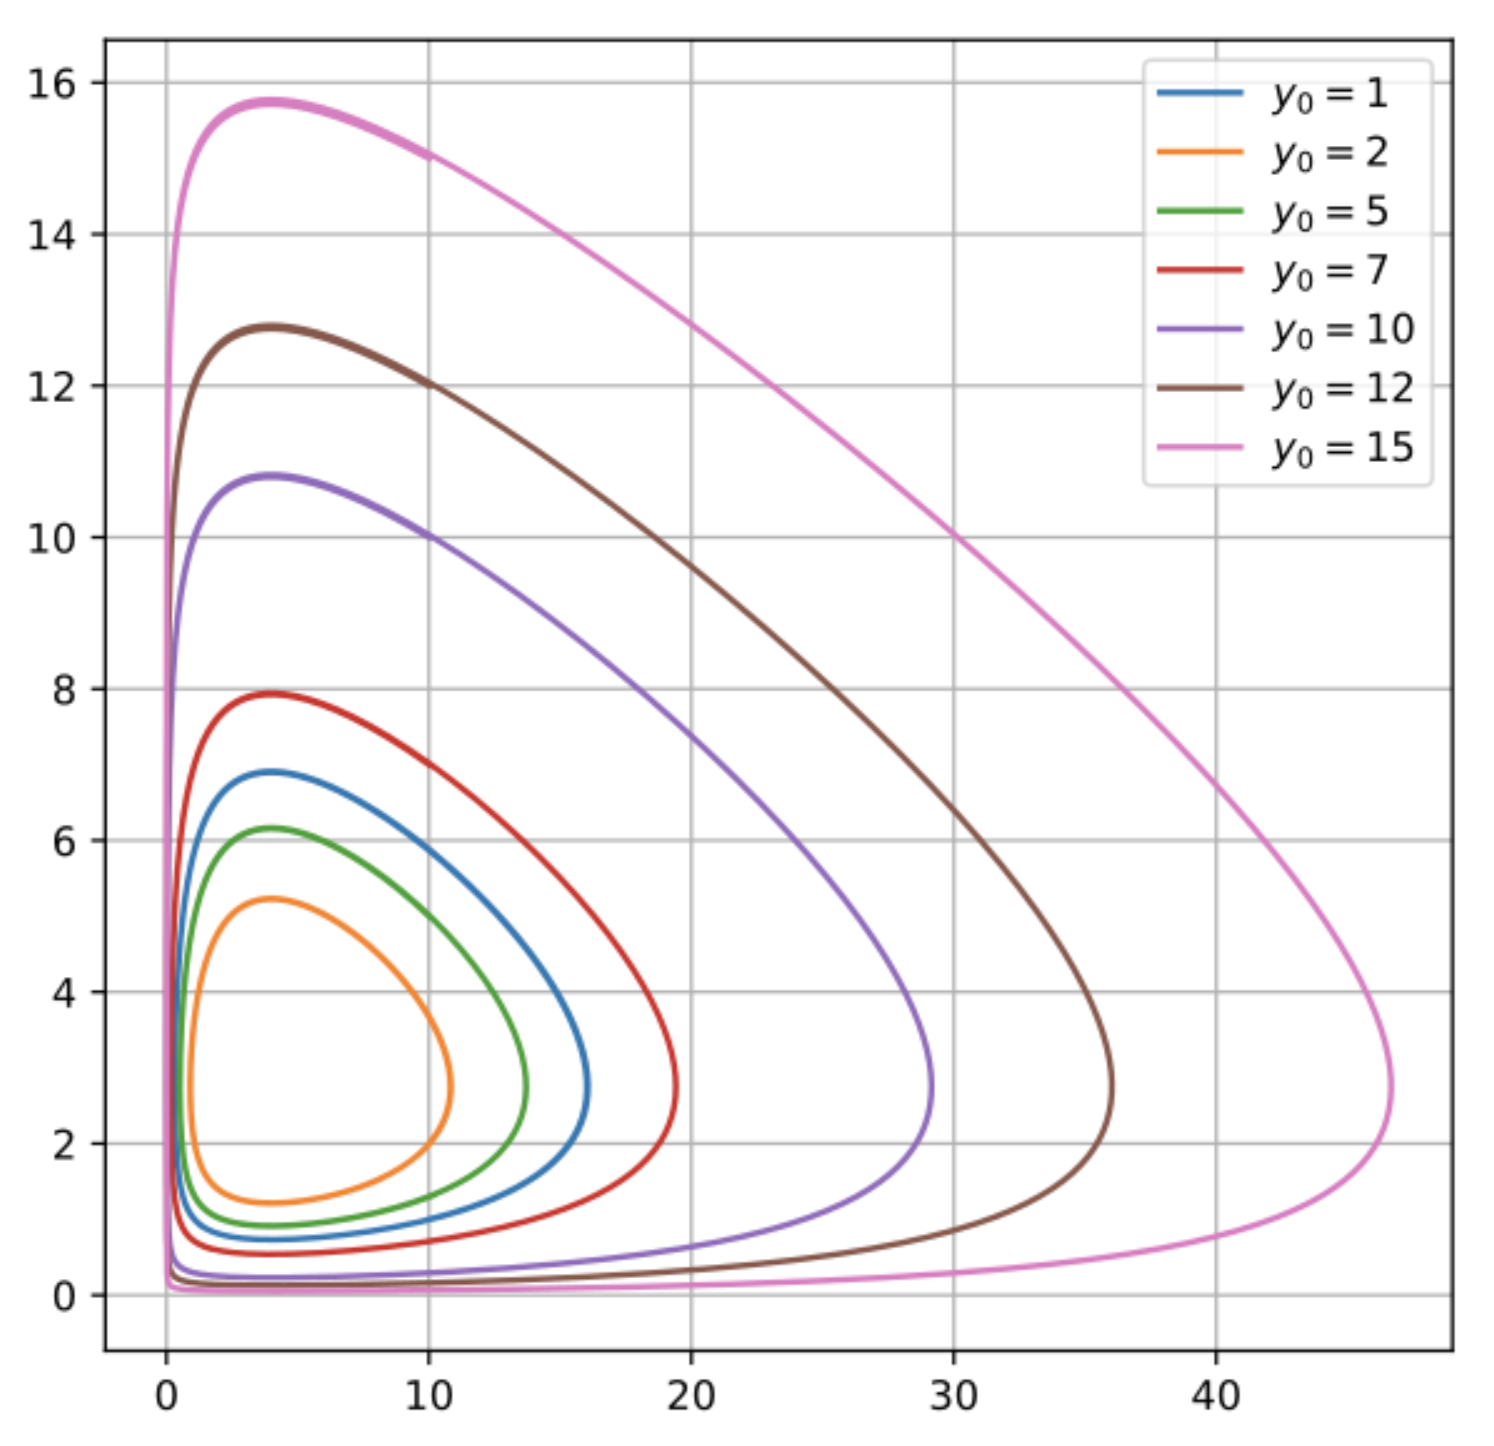
\includegraphics[width=0.4\linewidth]{../ExtFiles/LotkaVolteraSolns.png}
            \caption{Lotka-Volterra solution curves.}
            \label{fig:LotkaVolteraSolns}
        \end{figure}
        \begin{itemize}
            \item We have that
            \begin{align*}
                r' &= k_1r-awr&
                w' &= -k_2w+bwr
            \end{align*}
            where $r$ is rabbits and $w$ is wolves.
            \item We can rename the variables to
            \begin{equation*}
                \begin{cases}
                    x' = Ax-Bxy\\
                    y' = -Cy+Dxy
                \end{cases}
            \end{equation*}
            \item Dividing, we get
            \begin{align*}
                \frac{x'}{y'} &= \frac{Ax-Bxy}{-Cy+Dxy}\\
                \frac{Dx-C}{x}x'+\frac{By-A}{y}y' &= 0
            \end{align*}
            \item We seek a constant function $F:\R^2\to\R$ such that
            \begin{align*}
                \pdv{F}{x} &= \frac{Dx-C}{x}&
                \pdv{F}{y} &= \frac{By-A}{y}
            \end{align*}
            where we are imagining $x,y$ to be both parameterized by $t$ and arguments of $F$.
            \begin{itemize}
                \item Rationale: As a \emph{constant} function, $F$ satisfies
                \begin{align*}
                    0 &= \dv{F}{t}\\
                    &= \pdv{F}{x}\dv{x}{t}+\pdv{F}{y}\dv{y}{t}
                \end{align*}
                \item Comparing terms with the modified L-V equation yields the above PDEs.
            \end{itemize}
            \item We can solve the PDEs separately in this case to determine that $F$ is given by the following.
            \begin{align*}
                \dv{t}(Dx(t)-C\log x(t))+\dv{t}(By(t)-A\log y(t)) &= 0\\
                Dx(t)-C\log x(t)+By(t)-A\log y(t) &= E
            \end{align*}
            \begin{itemize}
                \item Much more on these machinations later; they are very important, though.
            \end{itemize}
            \item Alternative perspective on the above machinations:
            \begin{itemize}
                \item Assuming $y'\neq 0$, the original $x'/y'$ expression is equivalent to a separable differential equation in $\dv*{x}{y}$. Think
                \begin{equation*}
                    \dv{x}{y} = \frac{\dv*{x}{t}}{\dv*{y}{t}}
                \end{equation*}
                \item ...
            \end{itemize}
            \item Shao sketches some of the trajectories (they're all closed curves in the $xy$-plane). See Figure \ref{fig:LotkaVolteraSolns}
            \item Properties of the curves:
            \begin{itemize}
                \item The implicit relation which determines them: By the implicit function theorem, the $y$-derivative of the LHS is $B-A/y$ and the $x$-derivative of the LHS is $D-C/x$. Where the partial derivatives are equal to zero --- $(C/D,A/B)$ --- is interesting; it is a fixed point. Turning points happen when the $y$-coordinate is $A/B$ or the $x$-coordinate is $C/D$; note that the implicit function theorem fails here.
            \end{itemize}
        \end{itemize}
    \end{enumerate}
    \item \textbf{Finite lifespan}: Even if the RHS of $\dv*{y}{t}=f(t,y)$ is very regular, the solution can still blow up at some finite time.
    \item \textbf{Lifespan} (of a solution): How long the solution stays regular from the time that the evolution starts.
    \item \textbf{Interval of existence} (of a solution): The set of times $t$, starting from $t_0$, for which the solution stays regular.
    \item Lifespan vs. interval of existence: Essentially, if start time for a solution to an ODE is $t_0$ and the time at and beyond which the solution is no longer regular is $t_1\leq\infty$, then the lifespan is $t_1-t_0\leq\infty$ and the interval of existence is $[t_0,t_1)$.
    \item Consider the final ODE from the Brachistochrone problem.
    \begin{equation*}
        \dv{y}{x} = \sqrt{\frac{B-y}{y}}
    \end{equation*}
    \begin{itemize}
        \item Finding the \textbf{primitives}.
        \begin{itemize}
            \item What are these "primitives" Shao keeps talking about??
        \end{itemize}
        \item We should have
        \begin{equation*}
            \int\sqrt{\frac{y}{B-y}}\dd{y} = x
        \end{equation*}
        \item Change of variables: $y=B\sin^2\phi$ and $\dd{y}=2B\cos\phi\sin\phi\dd{\phi}$. Thus,
        \begin{equation*}
            \int\sqrt{\frac{y}{B-y}}\dd{y} = \int\frac{\sin\phi}{\cos\phi}\cdot 2B\cos\phi\sin\phi\dd{\phi}
            = 2B\int\sin^2\phi\dd{\phi}
        \end{equation*}
        \item The solution is
        \begin{equation*}
            \begin{cases}
                x = B\phi-\frac{B}{2}\sin(2\phi)+C\\
                y = B\sin^2\phi
            \end{cases}
        \end{equation*}
        \begin{itemize}
            \item If we set $2\phi=\theta$, then this is a parameterization of a cycloid.
        \end{itemize}
    \end{itemize}
    \item Later in the week, we will do SHM, the pendulum, the Kepler 2-body problem, and the Michaelis-Menten equation.
    \item Separable ODEs are a subset of ODEs of \textbf{exact form}.
    \item ODEs of exact form are of the form
    \begin{equation*}
        g(x,y)\dv{y}{x}+f(x,y) = 0
    \end{equation*}
    where for some $F(x,y)$, $g=\pdv*{F}{y}$, $f=\pdv*{F}{x}$, and partials commute. Equivalently,
    \begin{equation*}
        \pdv{g}{x} = \pdv{f}{y}
    \end{equation*}
    is our necessary and sufficient condition.
    \item By the law of composite differentiation,
    \begin{align*}
        \dv{x}\left[ F(x,y(x)) \right] &= \pdv{F}{x}(x,y(x))+\pdv{F}{y}(x,y(x))\cdot y'(x)\\
        &= f(x,y(x))+g(x,y(x))y'(x)\\
        &= 0
    \end{align*}
    \begin{itemize}
        \item Thus, there exists $C\in\R$ such that $F(x,y)=C$ along the entire set of solutions $(x,y)$. If an initial condition $(x_0,y_0)$ is given, we have in particular that $F(x_0,y_0)=C$. Thus, $F(x,y)=F(x_0,y_0)$ defines the solution corresponding to the aforementioned initial conditions implicitly.
        \item We solve these with an integrating factor $\mu\neq 0$ such that $(\mu g,\mu f)$ satisfy the constraint.
    \end{itemize}
\end{itemize}



\section{Office Hours (Shao)}
\begin{itemize}
    \item \textbf{Primitive}: An antiderivative.
    \item \textbf{Law of composite differentiation}: The chain rule.
    \item Went over how Shao has been applying the law of composite differentiation with respect to separable ODEs:
    \begin{itemize}
        \item Rearrange the initial separable ODE as follows.
        \begin{equation*}
            \frac{1}{g(y)}\cdot\dv{y}{t} = f(t)
        \end{equation*}
        \item Define $\dv*{H}{y}=1/g(y)$. Then, continuing from the above, we have by the law of composite differentiation that
        \begin{align*}
            \dv{H}{y}\cdot\dv{y}{t} &= f(t)\\
            \dv{H}{t} &= f(t)
        \end{align*}
        \item From the definition of $H$, we know that $H(y)=\int_{y_0}^y\dd{w}/g(w)$. We also have from the FTC that $f(t)=\dv{t}\int_{t_0}^tf(\tau)\dd{\tau}$. Thus, continuing from the above, we have that
        \begin{align*}
            \dv{t}(H) &= f(t)\\
            \dv{t}\left[ \int_{y_0}^y\frac{\dd{w}}{g(w)} \right] &= \dv{t}\int_{t_0}^tf(\tau)\dd{\tau}\\
            \dv{t}\left[ \int_{y_0}^{y(t)}\frac{\dd{w}}{g(w)}-\int_{t_0}^tf(\tau)\dd{\tau} \right] &= 0
        \end{align*}
        as desired.
        \item It follows that there exists $C\in\R$ such that
        \begin{equation*}
            \int_{y_0}^{y(t)}\frac{\dd{w}}{g(w)}-\int_{t_0}^tf(\tau)\dd{\tau} = C
        \end{equation*}
        for all $t$.
        \item In particular, if we choose $t=t_0$, then we can determine that
        \begin{equation*}
            C = \int_{y_0}^{y(t_0)}\frac{\dd{w}}{g(w)}-\int_{t_0}^{t_0}f(\tau)\dd{\tau}
            = \int_{y_0}^{y_0}\frac{\dd{w}}{g(w)}-0
            = 0
        \end{equation*}
        \item Therefore,
        \begin{equation*}
            \int_{y_0}^{y(t)}\frac{\dd{w}}{g(w)} = \int_{t_0}^tf(\tau)\dd{\tau}
        \end{equation*}
    \end{itemize}
    \item Take away from Brachistochrone problem:
    \begin{itemize}
        \item Just an example of a BDE; we won't have to answer questions on it.
    \end{itemize}
\end{itemize}



\section{ODEs of Exact Form}
\begin{itemize}
    \item \marginnote{10/5:}Last time, we discussed separable ODEs.
    \item Today, we will study \textbf{exact form} equations, as briefly touched on last class.
    \item \textbf{Exact form} (ODE): An ODE of the form
    \begin{equation*}
        g(x,y)\dv{y}{x}+f(x,y) = 0
    \end{equation*}
    where
    \begin{equation*}
        \pdv{g}{x} = \pdv{f}{y}
    \end{equation*}
    \begin{itemize}
        \item For equations of this form, there exists $F(x,y)$ such that
        \begin{align*}
            \pdv{F}{x} &= f&
            \pdv{F}{y} &= g&
            F(x,y(x)) &= C
        \end{align*}
        for some $C\in\R$.
        \item The scalar unknown function $y$ is allowed to take complex value here, but not generic vector value.
    \end{itemize}
    \item \textbf{Integrating factor}: A number or function $\mu$ such that
    \begin{align*}
        \mu g\dv{y}{x}+\mu f &= 0&
        \pdv{x}(\mu g) &= \pdv{y}(\mu f)
    \end{align*}
    \item Solving linear homogeneous equations of the form
    \begin{equation*}
        \dv{y}{t} = p(t)y
    \end{equation*}
    \begin{itemize}
        \item The solution is of the form
        \begin{equation*}
            y(t) = y_0\exp[\int_{t_0}^tp(\tau)\dd\tau]
        \end{equation*}
        \item The uniqueness of the solution follows from that of general separable equations.
    \end{itemize}
    \item Recall that $\e[a+ib]=\e[a](\cos b+i\sin b)$, so
    \begin{align*}
        \e[ix] &= \cos x+i\sin x&
        \cos x &= \frac{1}{2}(\e[ix]+\e[-ix])&
        \sin x &= \frac{1}{2i}(\e[ix]-\e[-ix])
    \end{align*}
    \item Example: If $y'=ky$, then $y'=-\lambda y$.
    \begin{itemize}
        \item What is this for??
    \end{itemize}
    \pagebreak
    \item Solving inhomogeneous linear equations of the form
    \begin{equation*}
        \dv{y}{t} = p(t)y+f(t)
    \end{equation*}
    \begin{itemize}
        \item Rewrite to
        \begin{equation*}
            1\cdot\dv{y}{t}+(-py-f) = 0
        \end{equation*}
        \item If the above equation is exact, it should satisfy the $\pdv*{g}{x}=\pdv*{f}{y}$ rule. To be more specific, in this case, we should have $\dv*{t}(1)=\dv*{y}(-py-f)$.
        \begin{itemize}
            \item Note that we switch from partial derivatives to ordinary derivatives because the specific equation we are considering only has two variables, total, at play ($y,t$ as opposed to $x,y,t$).
            \item Also note that we differentiate the LHS with respect to $t$ (instead of $x$) because the derivative in the rewritten form is with respect to $t$, and we base our formula on direct comparison.
        \end{itemize}
        \item However, we have
        \begin{equation*}
            \dv{t}(1) = 0 \neq -p(t) = \dv{y}(-p(t)y-f(t))
        \end{equation*}
        where $0\neq -p(t)$ in general (though there is a specific exception: $p(t)=0$).
        \begin{itemize}
            \item Thus, the above equation is \emph{not} exact. We will need to use integrating factors to make it so.
        \end{itemize}
        \item In particular, we wish to find an integrating factor $\mu(t,y)$ such that
        \begin{align*}
            \mu(t,y)\dv{y}{t}-\mu(t,y)p(t)y-\mu(t,y)f(t) &= 0&
            \dv{t}(\mu\cdot 1) &= \dv{y}(-\mu py-\mu f)
        \end{align*}
        \item By inspection, we can do this by taking $\mu$ to be a function of $t$, alone. Doing so, we obtain a linear homogeneous equation in $\mu$ that we can easily solve using the techniques from the previous example. Indeed, from the right equation above, we find
        \begin{align*}
            \dv{\mu}{t} &= \dv{y}(-\mu py-\mu f)\\
            \mu' &= -p(t)\mu\\
            \mu(t) &= \exp[-\int_{t_0}^tp(\tau)\dd\tau]
        \end{align*}
        \begin{itemize}
            \item Note that we may take the constant of integration/initial condition to be any number. Choosing 1, as we have above, is simply a matter of convenience.
        \end{itemize}
        \item If we let $P(t)=\int_{t_0}^tp(\tau)\dd\tau$, then
        \begin{align*}
            \e[-P(t)]y'(t)-p(t)\e[-P(t)]y(t) &= \e[-P(t)]f(t)\\
            \dv{t}(\e[-P(t)]y(t)) &= \e[-P(t)]f(t)\\
            \e[-P(t)]y(t)-\e[-P(t_0)]y(t_0) &= \int_{t_0}^t\e[-P(\tau)]f(\tau)\dd\tau
        \end{align*}
        \item Thus, we finally have the solution to the inhomogeneous problem as follows: The IVP $y'=py+f$, $y(t_0)=y_0$ has solution
        \begin{equation*}
            y(t) = y_0\e[P(t)-P(t_0)]+\e[P(t)]\int_0^t\e[-P(\tau)]f(\tau)\dd\tau
        \end{equation*}
        where $P$ is any anti-derivative of $p$.
        \item In particular, when $p(t)=a$, we get the \textbf{Duhamel formula} (which we should memorize).
    \end{itemize}
    \item \textbf{Duhamel formula}: The following equation, which is the solution to an inhomogeneous linear equation with $p(t)=a$.
    \begin{equation*}
        y(t) = y_0\e[a(t-t_0)]+\int_{t_0}^t\e[a(t-\tau)]f(\tau)\dd\tau
    \end{equation*}
    \begin{itemize}
        \item Important for computing forced oscillation.
    \end{itemize}
    \item Inspecting the inhomogeneous solution.
    \begin{itemize}
        \item The first term is the solution to the homogeneous form. The second term deals with the initial value.
    \end{itemize}
    \item Given an inhomogeneous equation, you can always write its solution as the combination of the solution to the homogeneous problem plus a particular solution, i.e.,
    \begin{equation*}
        y = y_h+y_p
    \end{equation*}
    \begin{itemize}
        \item "The general solution equals the homogeneous solution plus a particular solution."
        \item This is related to linear algebra, where the solution to $Ax=b$ is a particular solution $x_p$ plus any vector $x\in\ker A$.
        \item Thus, this idea will reappear in the theory of systems of linear ODEs.
    \end{itemize}
    \item We now look at systems of linear ODEs.
    \item Consider the harmonic oscillator: A particle of mass $m$ connected to an ideal spring (obeys Hooke's law) with no friction or gravity.
    \begin{itemize}
        \item Newton's second law: The acceleration is proportional to the restoring force.
        \item Hooke's law: The restoring force is of magnitude $kx$ in the opposite direction to the displacement.
        \item Thus, the ODE is of the form
        \begin{equation*}
            x'' = -\frac{k}{m}x
        \end{equation*}
        \item However, if there is damping (which will be proportional to the velocity), then the ODE is of the form
        \begin{equation*}
            x''+\frac{b}{m}x'+\frac{k}{m}x = 0
        \end{equation*}
    \end{itemize}
    \item We now address how to solve an ODE of the above form. In particular\dots
    \item Consider an ODE of the form
    \begin{equation*}
        y''+ay'+by = 0
    \end{equation*}
    for $a,b\in\C$.
    \begin{itemize}
        \item Rewrite the above differential equation in the following form.
        \begin{equation*}
            (y'-\mu y)'-\lambda(y'-\mu y) = 0
        \end{equation*}
        \begin{itemize}
            \item Shao never justifies how this rewrite may be derived. It appears to very much be "because it works" mathematics.
            \item Indeed, Shao claims that he figured it out himself when he was learning ODEs and could not point us to a reference source with a similar derivation when asked. He imagines it has been done previously, but does not know where off the top.
            \item In fact, this method is very much related to the classic approach to solving this ODE (transforming to a 2D system, calculating the eigenvalues [which are $\mu,\lambda$], and solving by linear combination). However, it is still clearly distinct. See also the first bonus problem from PSet 2.
        \end{itemize}
        \item Expanding, we can see that the above ODE is indeed equal to the original one, provided that we let $a=-(\mu+\lambda)$ and $b=\mu\lambda$.
        \begin{equation*}
            y''-(\mu+\lambda)y'+\mu\lambda y = 0
        \end{equation*}
        \item Now observe that under the above definitions of $\mu,\lambda$ in terms of $a,b$, we have that $\mu,\lambda$ are the roots of $x^2+ax+b=0$.
        \begin{align*}
            \mu^2-(\mu+\lambda)\mu+\mu\lambda &= 0&
            \lambda^2-(\mu+\lambda)\lambda+\mu\lambda &= 0&
        \end{align*}
        \begin{itemize}
            \item We call the binomial $x^2+ax+b=0$ the \textbf{characteristic polynomial} of the original ODE.
            \item Note that $\mu,\lambda$ can be complex (i.e., $\mu,\lambda\in\C$).
        \end{itemize}
        \item Substitute $x=y'-\mu y$. Then we can solve
        \begin{equation*}
            x'-\lambda x = 0
        \end{equation*}
        using the above methods to determine that $x=A\e[\lambda t]$.
        \item Returning the substitution, we have that
        \begin{equation*}
            y'-\mu y = A\e[\lambda t]
        \end{equation*}
        \item Since the above is of the form $y'=ay+f$, we can apply the Duhamel formula. It follows that the general solution is
        \begin{align*}
            y(t) &= B\e[\mu t]+\int_0^t\e[\mu(t-\tau)]A\e[\lambda\tau]\dd\tau\\
            &= B\e[\mu t]+A\e[\mu t]\int_0^t\e[(\lambda-\mu)\tau]\dd\tau
        \end{align*}
        for some $A,B\in\C$ dependent on the initial conditions.
        \item We now divide into two cases ($\mu\neq\lambda$ and $\mu=\lambda$).
        \begin{enumerate}
            \item ($\mu\neq\lambda$) Evaluating the above integral, we get
            \begin{align*}
                y(t) &= B\e[\mu t]+A\e[\mu t]\frac{\e[(\lambda-\mu)t]-1}{\lambda-\mu}\\
                &= B\e[\mu t]+\frac{A}{\lambda-\mu}\e[\lambda t]-\frac{A}{\lambda-\mu}\e[\mu t]\\
                &= \left( B-\frac{A}{\lambda-\mu} \right)\e[\mu t]+\frac{A}{\lambda-\mu}\e[\lambda t]\\
                &= A_1\e[\mu t]+B_1\e[\lambda t]
            \end{align*}
            where we define new constants $A_1,B_1\in\C$ in the last step for the sake of simplicity and WLOG. These new constants can be solved for just the same using the initial conditions.
            \item ($\mu=\lambda$) Since $\lambda-\mu=0$ in this case, the exponential function in the integral simplifies to unity. Therefore,
            \begin{align*}
                y(t) &= B\e[\mu t]+A\e[\mu t]\int_0^t1\dd\tau\\
                y(t) &= B\e[\mu t]+At\e[\mu t]\\
                &= A_1\e[\mu t]+B_1t\e[\mu t]
            \end{align*}
            where we define $A_1,B_1\in\C$ again for consistency with the above.
        \end{enumerate}
        \item These linearly independent solutions ($\e[\mu t]$ and $\e[\lambda t]$, or $\e[\mu t]$ and $t\e[\mu t]$) form a basis of the space of solutions; all solutions can be expressed as a linear combination of these two functions.
    \end{itemize}
    \item If our equation is of the form $y''+ay'+by=f(t)$, then we just need to apply the Duhamel formula twice (i.e., in the first step as well as the second step of the above derivation). In particular\dots
    \begin{itemize}
        \item Rewrite
        \begin{equation*}
            (y'-\mu y)'-\lambda(y'-\mu y) = f(t)
        \end{equation*}
        \item Substitute $x=y'-\mu y$ so that we have
        \begin{align*}
            x'-\lambda x &= f(t)\\
            x(t) &= A\e[\lambda t]+\int_0^t\e[\lambda(t-\tau)]f(\tau)\dd\tau
        \end{align*}
        \item Returning the substitution, we get
        \begin{align*}
            y'-\mu y &= A\e[\lambda t]+\int_0^t\e[\lambda(t-\tau_1)]f(\tau_1)\dd\tau_1\\
            y(t) &= B\e[\mu t]+\int_0^t\e[\mu(t-\tau_2)]\left( A\e[\lambda\tau_2]+\int_0^{\tau_2}\e[\lambda(\tau_2-\tau_1)]f(\tau_1)\dd\tau_1 \right)\dd\tau_2\\
            &= B\e[\mu t]+A\e[\mu t]\int_0^t\e[(\lambda-\mu)\tau_2]\dd\tau_2+\e[\mu t]\int_0^t\e[(\lambda-\mu)\tau_2]\int_0^{\tau_2}\e[-\lambda\tau_1]f(\tau_1)\dd\tau_1\dd\tau_2
        \end{align*}
        \item Notice how we have applied the Duhamel formula twice at this point (once in each of the last two steps).
        \item We once again divide into the two cases $\mu\neq\lambda$ and $\mu=\lambda$.
        \begin{enumerate}
            \item ($\mu\neq\lambda$) We have
            \begin{equation*}
                y(t) = A_1\e[\mu t]+B_1\e[\lambda t]+\e[\mu t]\int_0^t\e[(\lambda-\mu)\tau_2]\int_0^{\tau_2}\e[-\lambda\tau_1]f(\tau_1)\dd\tau_1\dd\tau_2
            \end{equation*}
            \item ($\mu=\lambda$) We have
            \begin{equation*}
                y(t) = A_1\e[\mu t]+B_1t\e[\mu t]+\e[\mu t]\int_0^t\int_0^{\tau_2}\e[-\mu\tau_1]f(\tau_1)\dd\tau_1\dd\tau_2
            \end{equation*}
        \end{enumerate}
        \item Notice how the left two terms in the final equations above are the homogeneous solutions derived previously, and the rightmost terms above are particular solutions.
    \end{itemize}
    \item Returning to the simple harmonic oscillator problem, we substitute $\omega=\sqrt{k/m}$ to get
    \begin{equation*}
        x'' = \omega^2x
    \end{equation*}
    \begin{itemize}
        \item The characteristic polynomial is
        \begin{equation*}
            0 = x^2+\omega^2
            = (x+i\omega)(x-i\omega)
        \end{equation*}
        \item Thus, solutions are of the form
        \begin{equation*}
            x = A_1\e[i\omega t]+B_1\e[-i\omega t]
        \end{equation*}
        \item It follows that the period is $T=2\pi/\omega$.
        \item To get a real (usable) solution, apply Euler's formula to get
        \begin{align*}
            x(t) &= A_1(\cos\omega t+i\sin\omega t)+B_1(\cos\omega t-i\sin\omega t)\\
            &= A\cos\omega t+B\sin\omega t
        \end{align*}
        where $A=A_1+B_1$, $B=iA_1-iB_1$.
        \item To match the initial condition $x(0)=x_0$, $x'(0)=v_0$, we use
        \begin{equation*}
            x(t) = x_0\cos\omega t+\frac{v_0}{\omega}\sin\omega t
        \end{equation*}
        \item In other words,
        \begin{align*}
            &
            \begin{cases}
                A=x_0\\
                \omega B=v_0
            \end{cases}
            &&
            \begin{cases}
                A_1+B_1=x_0\\
                i\omega A_1-i\omega B_1=v_0
            \end{cases}
        \end{align*}
        so
        \begin{align*}
            &
            \begin{cases}
                A=x_0\\
                B=\frac{v_0}{\omega}
            \end{cases}
            &&
            \begin{cases}
                A_1=\frac{1}{2}\left[ x_0-\frac{iv_0}{\omega} \right]\\
                B_1=\frac{1}{2}\left[ x_0+\frac{iv_0}{\omega} \right]
            \end{cases}
        \end{align*}
    \end{itemize}
\end{itemize}



\section{ODE Examples}
\begin{itemize}
    \item \marginnote{10/7:}Today, we will investigate a variety of examples of ODEs arising in real life.
    \item Michaelis-Menten kinetics: If E is an enzyme, S is its substrate, and P is the product, then the mechanism is
    \begin{equation*}
        \ce{E + S <=>[$k_1$][$k_{-1}$] ES ->[$k_2$] E + P}
    \end{equation*}
    \item The concentrations that we are concerned with are $\cnc{E},\cnc{S},\cnc{ES},\cnc{P}$.
    \item From the above mechanism, we can write the four rate laws
    \begin{align*}
        \dv{t}\cnc{S} &= -k_1\cnc{E}\cnc{S}+k_{-1}\cnc{ES}\tag{1}\\
        \dv{t}\cnc{E} &= -k_1\cnc{E}\cnc{S}+(k_{-1}+k_2)\cnc{ES}\tag{2}\\
        \dv{t}\cnc{ES} &= k_1\cnc{E}\cnc{S}-(k_{-1}+k_2)\cnc{ES}\tag{3}\\
        \dv{t}\cnc{P} &= k_2\cnc{ES}\tag{4}
    \end{align*}
    \item The initial conditions are $\cnc{S}=\cnc[0]{S}$ and $\cnc{E}=\cnc[0]{E}$.
    \item We can reduce these rate laws to the 2D system
    \begin{align*}
        \dv{t}\cnc{S} &= -k_1(\cnc[0]{E}-\cnc{ES})\cnc{S}+k_{-1}\cnc{ES}\tag{5}\\
        \dv{t}\cnc{ES} &= k_1(\cnc[0]{E}-\cnc{ES})\cnc{S}-(k_{-1}+k_2)\cnc{ES}\tag{6}
    \end{align*}
    \begin{itemize}
        \item Note that to do so, we have used two conservation laws: The conservation of the enzyme plus enzyme-substrate complex, and the conservation of the substrate plus enzyme-substrate complex plus products.
    \end{itemize}
    \item QSSA: Quasi steady-state assumption.
    \begin{itemize}
        \item Assume that $\cnc[0]{E}/\cnc[0]{S}\lll 1$.
        \item It follows that $\dv*{\cnc{ES}}{t}\approx 0$ due to saturation of the enzyme and $\cnc{S}\approx\cnc[0]{S}$ due to ever-more substrate being available.
    \end{itemize}
    \item Then
    \begin{equation*}
        \cnc{ES} = \frac{\cnc[0]{E}\cnc{S}}{K_M+\cnc{S}}
    \end{equation*}
    where $k_M=(k_{-1}+k_2)/k_1$ is the \textbf{Michaelis-Menten constant}, a usual indication of enzyme activity.
    \item Substitute the above into Equation 5:
    \begin{equation*}
        \dv{t}\cnc{S} = -\frac{v_\text{max}\cnc{S}}{k_M+\cnc{S}}
    \end{equation*}
    \begin{itemize}
        \item Note that $v_\text{max}=k_2\cnc[0]{E}$.
    \end{itemize}
    \item The above is now a differential equation of separable form; it's solution is
    \begingroup
    \allowdisplaybreaks
    \begin{align*}
        \int_{\cnc[0]{S}}^{\cnc{S}}-\frac{(k_M+z)\dd{z}}{zv_\text{max}} &= \int_0^t\dd{t}\\
        -\frac{k_M}{v_\text{max}}\log\frac{\cnc{S}}{\cnc[0]{S}}-\frac{1}{v_\text{max}}(\cnc{S}-\cnc[0]{S}) &= t\\
        \log\frac{\cnc{S}}{\cnc[0]{S}}+\frac{\cnc{S}}{k_M} &= \frac{\cnc[0]{S}-v_\text{max}t}{k_M}\\
        \frac{\cnc{S}}{\cnc[0]{S}}\e[\cnc{S}/k_M] &= \exp(\frac{\cnc[0]{S}-v_\text{max}t}{k_M})\\
        \frac{\cnc{S}}{k_M}\e[\cnc{S}/k_M] &= \frac{\cnc[0]{S}}{k_M}\exp(\frac{\cnc[0]{S}-v_\text{max}t}{k_M})\\
        \frac{\cnc{S}}{k_M} &= W\left[ \frac{\cnc[0]{S}}{k_M}\exp(\frac{\cnc[0]{S}-v_\text{max}t}{k_M}) \right]\\
        \cnc{S} &= k_MW\left[ \frac{\cnc[0]{S}}{k_M}\exp(\frac{\cnc[0]{S}-v_\text{max}t}{k_M}) \right]
    \end{align*}
    \endgroup
    \begin{itemize}
        \item Getting from line 5-6 (i.e., the introduction of $W$): Suppose we have an equation of the form $y\e[y]=x$. We cannot express $x$ in terms of $y$ using elementary functions, so we must define $W$ such that $y=W(x)$. Explicitly, $W$ is the unique function of $x$ that satisfies $W(x)\e[W(x)]=x$.
    \end{itemize}
    \item Harmonic oscillator.
    \item Recall that
    \begin{equation*}
        x''+\frac{k}{m}x = 0
    \end{equation*}
    \item Substituting $\omega=\sqrt{k/m}$, we can solve the above for
    \begin{equation*}
        x(t) = x(0)\cos(\omega t)+\frac{x'(0)}{\omega}\sin(\omega t)
    \end{equation*}
    \item This is an integrable system with $n$ degrees of freedom and $n-1$ scalar conservation laws??
    \item Conservation of mechanical energy:
    \begin{equation*}
        E = \frac{1}{2}m|x'|^2+\frac{1}{2}kx^2
    \end{equation*}
    \begin{figure}[h!]
        \centering
        \begin{tikzpicture}
            \footnotesize
            \draw
                (-3,0) -- (3,0) node[right]{$x$}
                (0,-2) -- (0,2) node[above]{$x'$}
            ;

            \draw [rex,thick]
                ellipse (6mm and 4mm)
                ellipse (12mm and 8mm)
                ellipse (18mm and 12mm)
            ;
        \end{tikzpicture}
        \caption{Conservation of mechanical energy in the harmonic oscillator.}
        \label{fig:harmonicEConservation}
    \end{figure}
    \begin{itemize}
        \item Differentiating wrt. $x$ yields
        \begin{align*}
            0 &= mx'x''+kxx'\\
            &= \dv{t}(\frac{1}{2}m(x')^2)+\dv{t}(\frac{1}{2}kx^2)
        \end{align*}
        \item This means that the solution is an ellipse in the $xx'$-plane, where each ellipse corresponds to an initial displacement and velocity.
    \end{itemize}
    \item Mathematical pendulum.
    \item Equation of motion:
    \begin{align*}
        0 &= l\theta''+g\sin\theta\\
        &= \ell\theta''\theta'+g\sin\theta\cdot\theta'\\
        &= \dv{t}\bigg( \underbrace{\frac{\ell}{2}|\theta'|^2-g\cos\theta}_E \bigg)
    \end{align*}
    \item Initial values:
    \begin{align*}
        \theta(0) &= \theta_0&
        \theta'(0) &= 0
    \end{align*}
    \item It follows from the above that
    \begin{align*}
        \frac{\ell}{2}|\theta'|^2-g\cos\theta_0 &= -g\cos\theta\\
        \dv{\theta}{t} &= \sqrt{\frac{2g}{\ell}(\cos\theta_0-\cos\theta)}\\
        \int_{\theta_0}^\theta\sqrt{\frac{\ell}{2g(\cos\theta_0-\cos\phi)}}\dd\phi &= t
    \end{align*}
    \begin{itemize}
        \item This is an elliptical integral (and thus cannot be expressed in terms of the elementary functions).
    \end{itemize}
    \item Suppose $\theta_0$ is small. Then $\theta$ is small, and we can invoke the small angle approximation $\sin\theta\approx\theta$.
    \begin{itemize}
        \item This yields an approximate equation of motion:
        \begin{equation*}
            \ell\theta''+g\theta = 0
        \end{equation*}
        \item From here, we can determine that $\theta(t)\approx\theta_0\cos\sqrt{g/\ell}\cdot t$ and $T=2\pi\sqrt{\ell/g}$.
    \end{itemize}
    \item Kepler problem.
    \item Two bodies of mass $m_1,m_2$ are located at positions $x_1,x_2$ pulling on each other gravitationally.
    \begin{itemize}
        \item The force of attraction is a conservative central force.
        \item The potential between the two masses is a function of their distance, i.e, $U(|x_1-x_2|)$.
    \end{itemize}
    \item From Newton's second and third law, we get
    \begin{align*}
        m_1x_1'' &= U'(|x_1-x_2|)\frac{x_2-x_1}{|x_2-x_1|}&
        m_2x_2'' &= U'(|x_1-x_2|)\frac{x_1-x_2}{|x_1-x_2|}
    \end{align*}
    \begin{itemize}
        \item The derivative of potential is force.
        \item The vector term provides direction.
    \end{itemize}
    \item Conservation of momentum:
    \begin{align*}
        (m_1x_1+m_2x_2)'' &= 0\\
        m_1x_1'+m_2x_2' &= C
    \end{align*}
    \begin{itemize}
        \item Let $M=m_1+m_2$. Then the center of mass
        \begin{equation*}
            \frac{m_1}{M}x_1+\frac{m_2}{M}x_2
        \end{equation*}
        moves inertially (i.e., does not accelerate or decelerate; is a stable reference frame) --- we'll define it to be the origin.
    \end{itemize}
    \item Conservation of angular momentum:
    \begin{equation*}
        [m(x_1-x_2)'\times(x_1-x_2)]' = 0
    \end{equation*}
    \begin{itemize}
        \item $m=m_1m_2/(m_1+m_2)$.
        \item $\times$ indicates the cross product.
        \item $L=m(x_1-x_2)'\times(x_1-x_2)$.
    \end{itemize}
    \item It follows that $x_1-x_2$ is always in a fixed plane, which we may call the \textbf{horizon plane}.
    \item Conservation of mechanical energy:
    \begin{align*}
        mq''+U'(|q|)\frac{q}{|q|} &= 0\\
        \frac{m}{2}|q'|^2+U(|q|) &= E
    \end{align*}
    \begin{itemize}
        \item $q=x_1-x_2$.
    \end{itemize}
    \item Introduce polar coordinates $(r,\phi)$.
    \begin{itemize}
        \item Then $r^2\phi'=\ell_0$, $r=r(\phi)$, and $\dv*{r}{\phi}=r'(t)/\phi'(t)$.
        \item It follows that
        \begin{equation*}
            \frac{m}{2}(|r'|^2+|\phi'|^2)+U(r) = E
        \end{equation*}
        \item Since $U(r)=-Gm_1m_2/r$ for Newtonian gravity,
        \begin{equation*}
            \left( \dv{r}{\phi} \right)^2+r^2 = \frac{2GMr^3}{\ell_0^2}+\frac{2Er^4}{m\ell_0^2}
        \end{equation*}
        \item The substitution $\mu=1/r$ yields
        \begin{equation*}
            \left( \dv{\mu}{\phi} \right)^2+\mu^2 = \frac{2GM}{\ell_0^2}\mu+\frac{2E}{m\ell_0^2}
        \end{equation*}
        \item Differentiating again gives
        \begin{equation*}
            2\dv{\mu}{\phi}\dv[2]{\mu}{\phi}+2\mu\dv{\mu}{\phi} = \frac{2GM}{\ell_0^2}\dv{\mu}{\phi}
        \end{equation*}
        \item Substituting $\mu=\cos(t)$ gives
        \begin{equation*}
            \dv[2]{\mu}{\phi}+\mu-\frac{GM}{\ell_0^2} = 0
        \end{equation*}
        or
        \begin{equation*}
            r = \frac{1}{GM/\ell_0^2+\varepsilon\cos(\phi-\phi_0)}
        \end{equation*}
        \begin{itemize}
            \item This is a conic section!
        \end{itemize}
    \end{itemize}
    \item Thus, for example, we can calculate the precession of Mercury.
    \item Note that while we have determined the trajectory of our 2 bodies in terms of elementary functions, the $n$-body problem cannot be solved analytically.
\end{itemize}



\section{Chapter 1: Introduction}
\emph{From \textcite{bib:Teschl}.}
\subsection*{Section 1.3: First Order Autonomous Equations}
\begin{itemize}
    \item \marginnote{11/15:}We start with the simplest nontrivial case of a first-order autonomous equation:
    \begin{equation*}
        \dot{x} = f(x)
        ,\quad
        x(0) = x_0
    \end{equation*}
    \begin{itemize}
        \item Since the system is autonomous, we may let $t_0=0$ WLOG. Indeed, if $\phi(t)$ is a solution to an autonomous equation satisfying $\phi(0)=x_0$, then $\psi(t)=\phi(t-t_0)$ is a solution with $\psi(t_0)=x_0$.
    \end{itemize}
    \item Solving this ODE.
    \begin{itemize}
        \item Suppose $f(x_0)\neq 0$. Divide both sides by $f(x)$ and integrate from the initial conditions onward to yield
        \begin{equation*}
            \int_0^t\frac{\dot{x}(s)\dd{s}}{f(x(s))} = t
        \end{equation*}
        \item Define
        \begin{equation*}
            F(x) := \int_{x_0}^x\frac{\dd{y}}{f(y)}
        \end{equation*}
        \begin{itemize}
            \item Note that this is just the previous equation under the "$u$-substitution" $y(t)=x(t)$, $\dd{y}=\dot{x}(t)\dd{t}$, $y(0)=x(0)=x_0$, $y(t)=x$.
        \end{itemize}
        \item Thus, in our new notation, any possible solution $x$ to the ODE must satisfy $F(x(t))=t$. It follows that $F(x)$ is monotone near $x_0$. Thus, it can be inverted to yield the unique solution
        \begin{equation*}
            \phi(t) = F^{-1}(t)
            ,\quad
            \phi(0) = F^{-1}(0) = x_0
        \end{equation*}
    \end{itemize}
    \item Investigating the maximal interval on which $\phi$ is defined.
    \item We focus on the case where $f(x_0)>0$ to start. We will treat $f(x_0)=0$ later; $f(x_0)<0$ is analogous to this section and will not be directly treated.
    \item Definitions and terms.
    \begin{itemize}
        \item By the assumed continuity of $f$, there exists an interval $(x_1,x_2)\ni x_0$ on which $f$ is positive.
        \begin{itemize}
            \item It will be useful to mention now that we want $x_1,x_2$ to be the maximal such values, i.e., for example, if $x>x_2$, then $f(x)\leq 0$. We will not explicitly deal with this stipulation until later, though.
        \end{itemize}
        \item Define
        \begin{align*}
            T_+ &= \lim_{x\to{x_2}^-}F(x)&
            T_- &= \lim_{x\to{x_1}^+}F(x)
        \end{align*}
        \begin{itemize}
            \item By the definition of $F$, $T_+\in(0,\infty]$ and $T_-\in[-\infty,0)$.
            \item $T_+$ is the supremum of all values of $t$ over which the solution is defined. $T_-$ is the respective infimum.
        \end{itemize}
        \item It follows --- by the definitions of $F,\phi$ and the FTC --- that $\phi\in C^1((T_-,T_+))$.
        \item It additionally follows by the definitions of $T_\pm$ that
        \begin{align*}
            \lim_{t\to{T_+}^-}\phi(t) &= x_2&
            \lim_{t\to{T_-}^+}\phi(t) &= x_1
        \end{align*}
    \end{itemize}
    \item Limits on the domain of $\phi$.
    \begin{itemize}
        \item The above implies that $\phi$ is defined for all $t>0$ iff
        \begin{equation*}
            T_+ = \int_{x_0}^{x_2}\frac{\dd{y}}{f(y)} = +\infty
        \end{equation*}
        \begin{itemize}
            \item Equivalently, $\phi$ is defined for all $t>0$ iff $1/f(x)$ is \emph{not} integrable near $x_2$
        \end{itemize}
        \item Similarly, $\phi$ is defined for all $t<0$ iff $1/f(x)$ is \emph{not} integrable near $x_1$.
        \item What about if $T_+<\infty$ (i.e., is finite)? We divide into two cases ($x_2=+\infty$ or $x_2<+\infty$).
        \item If $x_2=+\infty$, then by one of the above limits, $\phi$ diverges to $+\infty$ as $t\to T_+$. Thus, $\phi$ naturally cannot be extended (in a continuous way) to $t>T_+$, and hence $\phi$ is only defined for $t\in[0,T_+)$.
        \item If $x_2<+\infty$, we divide into two subcases. First off, if $f(x_2)>0$ (contrary to our assumption above that $x_1,x_2$ are maximal), then we can extend the solution beyond $x_2$ and we must redefine everything. Otherwise, $f(x_2)=0$; here, we can always extend $\phi$ by setting $\phi(t)=x_2$ for $t\geq T_+$. There may actually be more than one possible extension, though --- see the below example with $f(x)=\sqrt{|x|}$.
    \end{itemize}
    \item Example: $f(x)=x$ and $x_0>0$.
    \begin{itemize}
        \item If $x_0>0$, then $f(x_0)=x_0>0$. Thus, we can define an interval of positivity; specifically, we can determine by inspecting the graph of $f$ that this interval is $(x_1,x_2)=(0,+\infty)$.
        \item By definition, we have that
        \begin{equation*}
            F(x) = \int_{x_0}^x\frac{\dd{x}}{x}
            = \ln(\frac{x}{x_0})
        \end{equation*}
        \item By inspecting the graph of the above, we can see that $F$ approaches $+\infty$ as $x\to x_2=+\infty$, and $F$ approaches $-\infty$ as $x\to x_1=0$. Thus,
        \begin{align*}
            T_+ &= +\infty&
            T_- &= -\infty
        \end{align*}
        \item Additionally, $F$ is readily invertible, with inverse
        \begin{equation*}
            \phi(t) = x_0\e[t]
        \end{equation*}
        \item Lastly, since $T_+=+\infty$, we have by the above that $\phi$ is defined for all $t>0$. Similarly, we have that $\phi$ is defined for all $t<0$. Therefore, the solution $\phi$ is globally defined (defined on all of $\R$). Moreover, we can show symmetrically that $\phi$ is a solution for all $x_0\in\R$.
    \end{itemize}
    \item Example: $f(x)=x^2$ and $x_0>0$.
    \begin{itemize}
        \item As before, we have $(x_1,x_2)=(0,+\infty)$.
        \item By definition,
        \begin{equation*}
            F(x) = \frac{1}{x_0}-\frac{1}{x}
        \end{equation*}
        \item Thus,
        \begin{align*}
            T_+ &= \frac{1}{x_0}&
            T_- &= -\infty
        \end{align*}
        \item Additionally,
        \begin{equation*}
            \phi(t) = \frac{x_0}{1-x_0t}
        \end{equation*}
        \item As before, $\phi$ is defined for all $t<0$. However, since $T_+$ is finite, we have some additional complications there. From the above, this is a case of $T_+<\infty$ and $x_2=+\infty$, so we know that we cannot extend $\phi$ to or beyond $1/x_0$.
    \end{itemize}
    \item The case where $f(x_0)=0$.
    \begin{itemize}
        \item We have a trivial solution $\phi(t)=x_0$ to the initial condition $x(0)=x_0$.
        \item This is, in fact, not the only solution. If there exists $\varepsilon>0$ for which
        \begin{equation*}
            \left| \int_{x_0}^{x_0+\varepsilon}\frac{\dd{y}}{f(y)} \right| < \infty
        \end{equation*}
        then there is another solution
        \begin{equation*}
            \varphi(t) = F^{-1}(t)
        \end{equation*}
        with $\varphi(0)=x_0$ which is different from $\phi$!
    \end{itemize}
    \item Example: $f(x)=\sqrt{|x|}$ and $x_0>0$.
    \begin{itemize}
        \item We have $(x_1,x_2)=(0,+\infty)$.
        \item By definition,
        \begin{equation*}
            F(x) = 2(\sqrt{x}-\sqrt{x_0})
        \end{equation*}
        where we have removed the absolute values under the radicals because everything is positive in $x_0>0$ land.
        \item Naturally, $\phi(t)=0$ is a solution.
        \item However, since choosing $\varepsilon=1$ yields
        \begin{equation*}
            \left| \int_0^{0+1}\frac{\dd{y}}{\sqrt{|y|}} \right| = [2\sqrt{y}]_0^1
            = 2
            < \infty
        \end{equation*}
        we have an additional solution as well.
        \item In particular, this additional solution reads
        \begin{equation*}
            \varphi(t) = \left( \sqrt{x_0}+\frac{t}{2} \right)^2\footnotemark
        \end{equation*}
        \footnotetext{Compare with $t^2/4$ from class.}
        \item Additionally, we can determine as in previous examples that
        \begin{align*}
            T_- &= -2\sqrt{x_0}&
            T_+ &= +\infty
        \end{align*}
        \item Furthermore, this is a case of $T_->-\infty$, $x_1>-\infty$, and $f(x_1)=0$. Thus, we can extend $\phi$ beyond $t=-2\sqrt{x_0}$ with $\phi(t):=x_1=0$.
        \item In fact, this is not actually the only only possible extension; we may also patch in other nontrivial solutions. For example,
        \begin{equation*}
            \tilde{\phi}(t) =
            \begin{cases}
                -\frac{(t-t_0)^2}{4} & t\leq t_0\\
                0 & t_0<t<t_1\\
                \frac{(t-t_1)^2}{4} & t_1\leq t
            \end{cases}
        \end{equation*}
        is a perfectly valid solution to the differential equation $\dot{x}=\sqrt{|x|}$ for $t_0\leq t_1\in\R$ arbitrary.
    \end{itemize}
    \item Takeaways.
    \begin{itemize}
        \item "Solutions might only exist locally in $t$, even for perfectly nice $f$" \parencite[11]{bib:Teschl}.
        \item "Solutions might not be unique" \parencite[11]{bib:Teschl}.
        \begin{itemize}
            \item Note, however, that it is the fact that $f(x)=\sqrt{|x|}$ is not differentiable at $x_0=0$ that causes the problems.
        \end{itemize}
    \end{itemize}
    \item Several good problems; could be quite helpful with cementing these concepts.
    \begin{itemize}
        \item Some of these problems are also repeats from PSet 1.
    \end{itemize}
\end{itemize}


\subsection*{Section 1.4: Finding Explicit Solutions}
\begin{itemize}
    \item Solving ODEs for explicit solutions is impossible in general unless the equation is of a particular form.
    \item This section: Classes of first-order ODEs which are explicitly solvable.
    \item Strategy: Find a change of variables that transforms the ODE into a solvable form.
    \item Linear equation.
    \begin{align*}
        \dot{x} &= a(t)x&
        \dot{x} &= a(t)x+g(t)
    \end{align*}
    \begin{itemize}
        \item The left equation above is the homogeneous linear equation, and the right equation above is the corresponding inhomogeneous linear equation.
        \item The general solution to the homogeneous linear equation is
        \begin{equation*}
            \phi(t) = x_0A(t,t_0)
        \end{equation*}
        where
        \begin{equation*}
            A(t,s) = \e[\int_s^ta(s)\dd{s}]
        \end{equation*}
        \item The general solution to the inhomogeneous linear equation is
        \begin{equation*}
            \phi(t) = x_0A(t,t_0)+\int_{t_0}^tA(t,s)g(s)\dd{s}
        \end{equation*}
    \end{itemize}
    \item Coordinate transformations in differential equations.
    \begin{itemize}
        \item Suppose we have the point $(t,x)$ in the product space of the independent and dependent variables of our differential equation. We may change it to new coordinates $(s,y)$ given by
        \begin{align*}
            s &= \sigma(t,x)&
            y &= \eta(t,x)
        \end{align*}
        \item To not lose information, we require this transformation (i.e., both $\sigma,\eta$??) to be a \textbf{diffeomorphism}.
        \item To transform $\phi(t)$ into a new function $\psi(s)$, we need to eliminate $t$ from
        \begin{align*}
            s &= \sigma(t,\phi(t))&
            \psi &= \eta(t,\phi(t))
        \end{align*}
        by solving $s=\sigma(t,\phi(t))$ for $t$.
        \item However, this is not always possible for a diffeomorphism $\sigma$; indeed, if $\sigma$ corresponds to a rotation of the graph $(t,\phi(t))$ of $\phi$, for example, the result might not be the graph of a function. Thus, we additionally require that $\sigma$ be a \textbf{fiber preserving transformation}
        \begin{equation*}
            s = \sigma(t)
        \end{equation*}
        \item Defining $\sigma$ this way means that we can always define a unique inverse transformation
        \begin{align*}
            t &= \tau(s)&
            x &= \xi(s,y)
        \end{align*}
        \item It follows by the chain rule (think about this more??) that $\phi(t)$ satisfies
        \begin{equation*}
            \dot{x} = f(t,x)
        \end{equation*}
        iff $\psi(s)=\eta(\tau(s),\phi(\tau(s)))$ satisfies
        \begin{equation*}
            \dot{y} = \dot{\tau}\left( {\pdv{\eta}{t}}(\tau,\xi)+\pdv{\eta}{x}(\tau,\xi)f(\tau,\xi) \right)
        \end{equation*}
        where $\tau=\tau(s)$ and $\xi=\xi(s,y)$.
        \begin{itemize}
            \item The above notation is ostensibly unambiguous (why??).
            \item The following derivation of the above makes more intuitive sense, but may be ambiguous??
            \begin{equation*}
                \dv{y}{s} = \dv{s}(y(t(s),x(t(s))))
                = \pdv{y}{t}\dv{t}{s}+\pdv{y}{x}\dv{x}{t}\dv{t}{s}
            \end{equation*}
        \end{itemize}
    \end{itemize}
    \item \textbf{Fiber preserving transformation}: A map that sends the fibers $t=\text{const}$ to the fibers $s=\text{const}$.
    \begin{itemize}
        \item I suppose we can view the set of solutions to an ODE as a fiber bundle over the space of initial values.
        \item Alternatively, I think what this map might be doing is using time as the base space and defining the fiber corresponding to a specific time $t$ to be equal to the set of $\phi(t)$ for all the different $\phi$ (which are in bijective correspondence with the set of initial values). This would make sense, because this would imply that we're only stretching or shrinking time, not mapping it over itself, which is where problems would arise.
    \end{itemize}
    \item We now apply the above transformational mechanics to solve differential equations.
    \item \textbf{Homogeneous} (nonlinear differential equation): An ODE of the following form. \emph{Given by}
    \begin{equation*}
        \dot{x} = f(x/t)
    \end{equation*}
    \item Solving homogeneous equations.
    \begin{itemize}
        \item Apply the change of variables $y=x/t$ for $t\neq 0$.
        \item Definitions from the above:
        \begin{align*}
            \eta(t,x) &= x/t&
            \sigma(t) &= t&
            \tau(s) &= s&
            \xi(s,y) &= sy
        \end{align*}
        \begin{itemize}
            \item The definition for $\eta$ follows straight from $\eta(t,x)=y=x/t$.
            \item Under this definition of $\eta$, we must choose $\sigma$ to be the identity to still have $y=x/t$. If, for example, we had chosen $\tilde{\eta}(t,x)=x/2t$, then we would have needed to choose $\tilde{\sigma}(t)=2t$. This would have made it so that $y(s)=x/2t=x/s$, as desired.
            \item $\tau$ is the straightforward inverse of the identity $\sigma$, and hence still the identity.
            \item Under this definition of $\xi$, we can see that
            \begin{gather*}
                y = \eta(\tau(s),\xi(s,y))
                    = \frac{\xi(s,y)}{\tau(s)}
                    = \frac{sy}{s}
                    = y\\
                x = \xi(\sigma(t),\eta(t,x))
                    = \sigma(t)\cdot\eta(t,x)
                    = t\cdot\frac{x}{t}
                    = x
            \end{gather*}
            Therefore, $\xi$ is an appropriate inverse.
        \end{itemize}
        \item It follows by the above that our new differential equation is
        \begin{align*}
            \dot{y} &= \dot{\tau}\left( {\pdv{\eta}{t}}(\tau,\xi)+\pdv{\eta}{x}(\tau,\xi)f(\tau,\xi) \right)\\
            &= 1\cdot\left( \left[ -\frac{x}{t^2} \right]_{(t,x)=(s,sy)}+\left[ \frac{1}{t} \right]_{(t,x)=(s,sy)}\cdot f(\xi/\tau) \right)\\
            &= -\frac{sy}{s^2}+\frac{1}{s}\cdot f(y)\\
            &= \frac{f(y)-y}{s}
        \end{align*}
        \begin{itemize}
            \item Recall that since the independent variable corresponding to $y$ is $s$, the Newtonian dot derivative denotes a derivative with respect to $s$.
        \end{itemize}
        \item This equation is separable.
    \end{itemize}
    \item \textcite{bib:Teschl} covers a more general form of homogeneous equations that may lend additional insight into cases where $\sigma$ is not the identity.
    \item \textbf{Bernoulli equation}: An ODE of following form. \emph{Also known as} \textbf{Bernoulli type} (ODE). \emph{Given by}
    \begin{equation*}
        \dot{x} = f(t)x+g(t)x^n
    \end{equation*}
    where $n\neq 0,1$.
    \begin{itemize}
        \item We exclude $n=0,1$ because in these cases, the equation is already linear.
    \end{itemize}
    \item Solving Bernoulli type ODEs.
    \begin{itemize}
        \item Use the transformation $y=x^{1-n}$.
        \item Then
        \begin{align*}
            \dot{y} &= \dot{\tau}\left( {\pdv{\eta}{t}}(\tau,\xi)+\pdv{\eta}{x}(\tau,\xi)f(\tau,\xi) \right)\\
            &= 1\cdot\left( [0]_{(s,y^{1/(1-n)})}+[(1-n)x^{-n}]_{(s,y^{1/(1-n)})}\cdot[f(\tau)\xi+g(\tau)\xi^n] \right)\\
            &= (1-n)y^{-n/(1-n)}[f(s)y^{1/(1-n)}+g(s)y^{n/(1-n)}]\\
            &= (1-n)f(s)y+(1-n)g(s)
        \end{align*}
        \item This is now a readily solvable linear equation.
    \end{itemize}
    \item \textbf{Riccati equation}: An ODE of the following form. \emph{Also known as} \textbf{Riccati type} (ODE). \emph{Given by}
    \begin{equation*}
        \dot{x} = f(t)x+g(t)x^2+h(t)
    \end{equation*}
    \item Solving Riccati type ODEs.
    \begin{itemize}
        \item To solve these, you need a particular solution $x_p(t)$. Then, you can use the transformation
        \begin{equation*}
            y = \frac{1}{x-x_p(t)}
        \end{equation*}
        to yield the following linear equation.
        \begin{equation*}
            \dot{y} = -(f(s)+2x_p(s)g(s))y-g(s)
        \end{equation*}
    \end{itemize}
    \item Further clever transformations can be looked up in reference works.
    \item Rule of thumb: "For a first-order equation, there is a realistic chance that it is explicitly solvable. But already for second-order equations, explicitly solvable ones are rare" \parencite[16]{bib:Teschl}.
    \item Using Mathematica to help solve ODEs and gain an intuition for how they work (e.g., with slope fields or \textbf{directional fields}).
    \item Equations of exact form are covered in the problems to this section.
    \begin{itemize}
        \item Again, some of these problems are repeats from PSet 1.
    \end{itemize}
\end{itemize}



\section{Chapter 8: Higher Dimensional Dynamical Systems}
\emph{From \textcite{bib:Teschl}.}
\subsection*{Section 8.5: The Kepler Problem}
\begin{itemize}
    \item \marginnote{12/6:}I would need Hamiltonian mechanics (and hence boundary value problems) in order to understand this.
\end{itemize}




\end{document}